% answers.tex —— 1958 年·江苏卷 · 参考答案与详细解析片段
% 由 tools/generate_projects.py 依来源总账自 1958/1958_江苏_数学真题_试题.md + 1958/1958_江苏_数学真题_解析正文.md + 1958/1958_江苏_数学真题_答案要点.md 生成，勿手改（改源 MD 后重跑）


\begin{gktip}
本卷题面出自固定原卷（仅题面，无答案页）；以下解析由本库逐题独立推导，不声称代表官方发布版本。两点约定：第 1 题第（2）小问按角度制把 $10^{x}$ 理解为以「度」计的角；第 5 题原卷未定义 $a$、$b$、$c$，按通行约定取 $AD=a$、$DC=b$、$CB=c$（见试题源注）。
\end{gktip}

\begin{answer}
\gksolhead{1}{}

\textbf{题目}：

解下列各题：

（1） 解方程 $\lg(x+7)-\lg(x+1)=\lg(x+3)$；

（2） 解方程 $\sin 10^{x}=\dfrac{1}{2}$；

（3） 设 $\tan\dfrac{\theta}{2}=t$，求证：$\tan\theta=\dfrac{2t}{1-t^{2}}$，$\sin\theta=\dfrac{2t}{1+t^{2}}$，$\cos\theta=\dfrac{1-t^{2}}{1+t^{2}}$。

\Needspace{4\baselineskip}
\textbf{解析}

\gksubpart{（1）}

依对数真数为正的要求：$x+7>0$，$x+1>0$，$x+3>0$，故定义域为 $x>-1$。

\Needspace{5\baselineskip}
原方程化为

\nopagebreak[4]
\[
\lg\frac{x+7}{x+1}=\lg(x+3)
\]

\Needspace{5\baselineskip}
由对数相等则真数相等：

\nopagebreak[4]
\[
\frac{x+7}{x+1}=x+3
\]

\Needspace{5\baselineskip}
去分母：

\nopagebreak[4]
\[
x+7=(x+1)(x+3)=x^{2}+4x+3
\]

\Needspace{5\baselineskip}
整理得

\nopagebreak[4]
\[
x^{2}+3x-4=0,\qquad (x-1)(x+4)=0
\]

\Needspace{5\baselineskip}
故 $x=1$ 或 $x=-4$。经定义域检验，$x=-4$ 使 $\lg(x+7)$、$\lg(x+1)$ 无意义，为增根，舍去。原方程的解为

\nopagebreak[4]
\[
x=1
\]

\gksubpart{（2）}

方程 $\sin 10^{x}=\dfrac{1}{2}$ 中的角按角度制理解：把 $10^{x}$ 看作以「度」计的角。

\Needspace{5\baselineskip}
由 $\sin\alpha=\dfrac{1}{2}$ 的一般解

\nopagebreak[4]
\[
10^{x}=30^{\circ}+360^{\circ}k\ \text{或}\ 150^{\circ}+360^{\circ}k\qquad(k\in\mathbb{Z})
\]

\Needspace{5\baselineskip}
而 $10^{x}>0$，故 $360k+30>0$、$360k+150>0$，即 $k\ge 0$。对两边取常用对数（取度数数值）得

\nopagebreak[4]
\[
x=\lg(360k+30)\ \text{或}\ x=\lg(360k+150)\qquad(k\ \text{为非负整数})
\]

\gksubpart{（3）}

\Needspace{5\baselineskip}
由倍角公式并用 $\sin^{2}\dfrac{\theta}{2}+\cos^{2}\dfrac{\theta}{2}=1$（分子分母同除 $\cos^{2}\dfrac{\theta}{2}$）：

\nopagebreak[4]
\[
\sin\theta=2\sin\frac{\theta}{2}\cos\frac{\theta}{2}
=\frac{2\sin\frac{\theta}{2}\cos\frac{\theta}{2}}{\sin^{2}\frac{\theta}{2}+\cos^{2}\frac{\theta}{2}}
=\frac{2\tan\frac{\theta}{2}}{1+\tan^{2}\frac{\theta}{2}}
=\frac{2t}{1+t^{2}}
\]

\Needspace{5\baselineskip}
同理

\nopagebreak[4]
\[
\cos\theta=\cos^{2}\frac{\theta}{2}-\sin^{2}\frac{\theta}{2}
=\frac{\cos^{2}\frac{\theta}{2}-\sin^{2}\frac{\theta}{2}}{\sin^{2}\frac{\theta}{2}+\cos^{2}\frac{\theta}{2}}
=\frac{1-t^{2}}{1+t^{2}}
\]

\Needspace{5\baselineskip}
相除得

\nopagebreak[4]
\[
\tan\theta=\frac{\sin\theta}{\cos\theta}
=\frac{2t}{1-t^{2}}
\]

\gkanswer{答案（1）：$x=1$}

\gkanswer{答案（2）：$x=\lg(360k+30)$ 或 $x=\lg(360k+150)$（$k$ 为非负整数；$10^{x}$ 按角度制理解）}

\gkanswer{答案（3）：见解析版}

\end{answer}
\begin{answer}
\gksolhead{2}{}

\textbf{题目}：

解方程 $\sin x+\sqrt{3}\cos x=2$。

\Needspace{4\baselineskip}
\textbf{解析}

\Needspace{5\baselineskip}
配辅助角：

\nopagebreak[4]
\[
\sin x+\sqrt{3}\cos x
=2\left(\frac{1}{2}\sin x+\frac{\sqrt{3}}{2}\cos x\right)
=2\sin\left(x+\frac{\pi}{3}\right)
\]

\Needspace{5\baselineskip}
方程化为

\nopagebreak[4]
\[
2\sin\left(x+\frac{\pi}{3}\right)=2,\qquad \sin\left(x+\frac{\pi}{3}\right)=1
\]

\Needspace{5\baselineskip}
故

\nopagebreak[4]
\[
x+\frac{\pi}{3}=\frac{\pi}{2}+2k\pi
\]

\Needspace{5\baselineskip}
即

\nopagebreak[4]
\[
x=\frac{\pi}{6}+2k\pi\qquad(k\in\mathbb{Z})
\]

\gkanswer{答案：$x=\dfrac{\pi}{6}+2k\pi$（$k$ 为整数）}

\end{answer}
\begin{answer}
\gksolhead{3}{}

\textbf{题目}：

已知正六棱锥底边长为 $a$，高为 $h$，求侧面积。

\Needspace{4\baselineskip}
\textbf{解析}

\Needspace{5\baselineskip}
正六边形的边长等于其外接圆半径，故基面中心到各顶点的距离为 $a$。设侧棱长为 $e$，则

\nopagebreak[4]
\[
e=\sqrt{h^{2}+a^{2}}
\]

\Needspace{5\baselineskip}
侧面等腰三角形的底边为 $a$，其斜高为

\nopagebreak[4]
\[
l=\sqrt{e^{2}-\left(\frac{a}{2}\right)^{2}}
=\sqrt{h^{2}+a^{2}-\frac{a^{2}}{4}}
=\sqrt{h^{2}+\frac{3a^{2}}{4}}
\]

\Needspace{5\baselineskip}
侧面积为 $6$ 个全等侧面三角形之和：

\nopagebreak[4]
\[
S_{\text{侧}}=6\cdot\frac{1}{2}a\,l
=3a\sqrt{h^{2}+\frac{3a^{2}}{4}}
=\frac{3a}{2}\sqrt{4h^{2}+3a^{2}}
\]

\gkanswer{答案：$S_{\text{\text{侧}}}=\dfrac{3a}{2}\sqrt{4h^{2}+3a^{2}}$}

\end{answer}
\begin{answer}
\gksolhead{4}{}

\textbf{题目}：

已知长方体三度的和为 $a+b+c=13$，对角线长为 $\sqrt{65}$，求全面积。

\Needspace{4\baselineskip}
\textbf{解析}

长方体对角线长的平方等于三度平方和：$a^{2}+b^{2}+c^{2}=65$。

\Needspace{5\baselineskip}
全面积为

\nopagebreak[4]
\[
S=2(ab+bc+ca)
\]

\Needspace{5\baselineskip}
利用恒等式

\nopagebreak[4]
\[
(a+b+c)^{2}=a^{2}+b^{2}+c^{2}+2(ab+bc+ca)
\]

\Needspace{5\baselineskip}
得

\nopagebreak[4]
\[
S=(a+b+c)^{2}-(a^{2}+b^{2}+c^{2})=13^{2}-65=169-65=104
\]

\gkanswer{答案：$104$}

\end{answer}
\begin{answer}
\gksolhead{5}{}

\textbf{题目}：

已知 $AB$ 为圆的直径，$DC$ 为圆的弦，四边形 $ABCD$ 内接于圆。

（1） 求证：$AC\cdot DB=AB\cdot DC+AD\cdot CB$；

（2） 求证：直径 $AB$ 为方程 $x^{3}-(a^{2}+b^{2}+c^{2})x-2abc=0$ 的根。
\nopagebreak[4]
\begin{center}% 1958 年江苏卷第 5 题：圆内接四边形 ABCD（AB 为水平直径，D、C 在上半圆，D 约 115°、C 约 56° 方向），连 AD、DC、CB 与对角线 AC、DB；源卷图无顶点圆点、无圆心标记，故不标（按源卷布局）
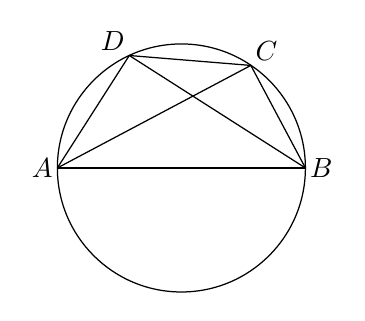
\begin{tikzpicture}[scale=1.05, line width=0.45pt,
  every node/.style={inner sep=1.5pt}]
  \coordinate (A) at (-1.5,0);
  \coordinate (B) at (1.5,0);
  \coordinate (D) at (-0.63,1.36);
  \coordinate (C) at (0.84,1.24);
  \draw (0,0) circle (1.5);
  \draw (A) -- (B);
  \draw (A) -- (D);
  \draw (D) -- (C);
  \draw (C) -- (B);
  \draw (A) -- (C);
  \draw (D) -- (B);
  \node[anchor=east] at (A) {$A$};
  \node[anchor=west] at (B) {$B$};
  \node[anchor=south east] at (D) {$D$};
  \node[anchor=south west] at (C) {$C$};
\end{tikzpicture}
\end{center}
\nopagebreak[4]
\begin{gktip}
\textbf{源注}：原卷未交代第（2）小问中 $a$、$b$、$c$ 的含义；按本题通行理解，系指 $AD=a$、$DC=b$、$CB=c$（解析依此进行），转录保留原卷写法。
\end{gktip}

\Needspace{4\baselineskip}
\textbf{解析}
\nopagebreak[4]
\begin{center}% 1958 年江苏卷第 5 题：圆内接四边形 ABCD（AB 为水平直径，D、C 在上半圆，D 约 115°、C 约 56° 方向），连 AD、DC、CB 与对角线 AC、DB；源卷图无顶点圆点、无圆心标记，故不标（按源卷布局）
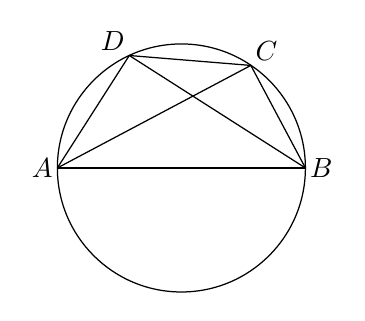
\begin{tikzpicture}[scale=1.05, line width=0.45pt,
  every node/.style={inner sep=1.5pt}]
  \coordinate (A) at (-1.5,0);
  \coordinate (B) at (1.5,0);
  \coordinate (D) at (-0.63,1.36);
  \coordinate (C) at (0.84,1.24);
  \draw (0,0) circle (1.5);
  \draw (A) -- (B);
  \draw (A) -- (D);
  \draw (D) -- (C);
  \draw (C) -- (B);
  \draw (A) -- (C);
  \draw (D) -- (B);
  \node[anchor=east] at (A) {$A$};
  \node[anchor=west] at (B) {$B$};
  \node[anchor=south east] at (D) {$D$};
  \node[anchor=south west] at (C) {$C$};
\end{tikzpicture}
\end{center}
\nopagebreak[4]
\gksubpart{（1）}

在第（1）小问的证明中不需要用到 $a$、$b$、$c$。

在 $AC$ 上取点 $E$，使 $\angle ADE=\angle BDC$。

\Needspace{5\baselineskip}
由同弧上的圆周角相等，$\angle DAE=\angle DAC=\angle DBC$（都对弧 $DC$），故

\nopagebreak[4]
\[
\triangle ADE\sim\triangle BDC
\]

\Needspace{5\baselineskip}
于是

\nopagebreak[4]
\[
\frac{AE}{CB}=\frac{AD}{BD}
\]

\Needspace{5\baselineskip}
即

\nopagebreak[4]
\[
AE\cdot BD=AD\cdot CB
\]

\Needspace{5\baselineskip}
又由 $\angle ADE=\angle BDC$ 得

\nopagebreak[4]
\[
\angle CDE=\angle CDA-\angle ADE=\angle CDA-\angle BDC=\angle BDA
\]

（射线 $DB$ 在 $\angle CDA$ 内部，$E$ 在 $AC$ 上使射线 $DE$ 也在 $\angle CDA$ 内部。）

\Needspace{5\baselineskip}
而 $\angle DCE=\angle DCA=\angle DBA$（都对弧 $DA$），故

\nopagebreak[4]
\[
\triangle CDE\sim\triangle BDA
\]

\Needspace{5\baselineskip}
于是

\nopagebreak[4]
\[
\frac{CE}{BA}=\frac{CD}{BD}
\]

\Needspace{5\baselineskip}
即

\nopagebreak[4]
\[
CE\cdot BD=AB\cdot DC
\]

\Needspace{5\baselineskip}
两式相加（$E$ 在线段 $AC$ 上，$AE+CE=AC$）：

\nopagebreak[4]
\[
BD\cdot(AE+CE)=AD\cdot CB+AB\cdot DC
\]

\Needspace{5\baselineskip}
即

\nopagebreak[4]
\[
AC\cdot DB=AB\cdot DC+AD\cdot CB
\]

这就是托勒密定理。

\gksubpart{（2）}

依约定取 $AD=a$，$DC=b$，$CB=c$，并设 $x=AB$。

\Needspace{5\baselineskip}
因 $AB$ 为直径，由直径上的圆周角是直角，$\angle ACB=\angle ADB=90^{\circ}$，故

\nopagebreak[4]
\[
AC^{2}=x^{2}-c^{2},\qquad DB^{2}=x^{2}-a^{2}
\]

\Needspace{5\baselineskip}
代入第（1）小问结论 $AC\cdot DB=AB\cdot DC+AD\cdot CB$：

\nopagebreak[4]
\[
\sqrt{x^{2}-c^{2}}\cdot\sqrt{x^{2}-a^{2}}=bx+ac
\]

\Needspace{5\baselineskip}
因 $bx+ac>0$，两边平方不产生增根：

\nopagebreak[4]
\[
(x^{2}-c^{2})(x^{2}-a^{2})=b^{2}x^{2}+2abcx+a^{2}c^{2}
\]

\Needspace{5\baselineskip}
展开：

\nopagebreak[4]
\[
x^{4}-(a^{2}+c^{2})x^{2}+a^{2}c^{2}=b^{2}x^{2}+2abcx+a^{2}c^{2}
\]

\Needspace{5\baselineskip}
消去 $a^{2}c^{2}$：

\nopagebreak[4]
\[
x^{4}-(a^{2}+b^{2}+c^{2})x^{2}-2abcx=0
\]

\Needspace{5\baselineskip}
即

\nopagebreak[4]
\[
x\left[x^{3}-(a^{2}+b^{2}+c^{2})x-2abc\right]=0
\]

\Needspace{5\baselineskip}
因 $x=AB>0$，约去 $x$ 得

\nopagebreak[4]
\[
x^{3}-(a^{2}+b^{2}+c^{2})x-2abc=0
\]

故直径 $AB$ 的长满足该方程，即 $AB$ 为方程 $x^{3}-(a^{2}+b^{2}+c^{2})x-2abc=0$ 的根。

\gkanswer{答案（1）：见解析版}

\gkanswer{答案（2）：见解析版}

\end{answer}